\section{Computer-assisted validation}
\label{sec:cap}

The proof of \cref{thm:principal} requires two finite-time facts about the same exact rational point IVP: the trajectory must be enclosed tightly enough to certify entry into the cold-start extinction strip, and the validated finite history must be accurate enough to certify the inherited memory term in \cref{thm:memory-tail}. A direct normwise fractional Grönwall estimate is too pessimistic for this orbit because it replaces the time-dependent matrix dynamics by absolute-value amplification. We therefore validate the computed trajectory by an orbit-linearized Volterra fixed-point argument.

\begin{figure}[t]
  \centering
  \resizebox{\textwidth}{!}{\begin{tikzpicture}[
  node distance=8mm and 12mm,
  box/.style={draw,rounded corners,align=center,minimum height=10mm,minimum width=31mm,font=\small},
  cert/.style={draw,rounded corners,align=center,minimum height=10mm,minimum width=31mm,font=\small,fill=black!8},
  arr/.style={->,thick}
]
  \node[box] (center) {numerical center\\and source residual};
  \node[box,right=of center] (inv) {orbit-linearized\\verified inverse};
  \node[cert,right=of inv] (close) {cellwise self-map\\+\ Perron contraction};

  \node[cert,below=13mm of inv] (tube) {unique exact\\trajectory tube};

  \node[cert,below left=12mm and 19mm of tube] (entry)
    {threshold entry\\feeds X1};
  \node[cert,below right=12mm and 19mm of tube] (tail)
    {validated history\\feeds M1};

  \draw[arr] (center)--(inv);
  \draw[arr] (inv)--(close);
  \draw[arr] (close.south) |- (tube.east);
  \draw[arr] (tube)--(entry);
  \draw[arr] (tube)--(tail);

  \node[font=\footnotesize,align=center,below=7mm of tube]
    {\(L_h=I-AW\), \qquad \(F(b)<b\), \qquad \(\kappa<1\)};
\end{tikzpicture}
}
  \caption{Logical architecture of the finite-history computer-assisted proof.  The sign-aware inverse is validated before nonnegative cellwise bounds are applied; the resulting exact state tube is then used independently for threshold entry and for the memory-tail constants.}
  \label{fig:cap-architecture}
\end{figure}

\subsection{Source correction equation}

Let the numerical center be written as
\[
  \widehat X(t)
  =
  p+I^\alpha\phi(t),
\]
where
\[
  (I^\alpha f)(t)
  =
  \frac1{\Gamma(\alpha)}
  \int_0^t(t-s)^{\alpha-1}f(s)\,ds.
\]
Define
\[
  \rho(t)
  =
  \phi(t)-g(\widehat X(t)).
\]
If
\[
  X=\widehat X+I^\alpha f,
\]
then the exact correction source \(f\) satisfies
\begin{equation}
  \mathcal H(f)
  =
  f-
  \left[
  g(\widehat X+I^\alpha f)-g(\widehat X)
  \right]
  +\rho
  =
  0.
  \label{eq:source-equation}
\end{equation}
At \(f=0\),
\[
  D\mathcal H(0)=I-K,
  \qquad
  (Kf)(t)=A(t)I^\alpha f(t),
\]
with
\[
  A(t)=Dg(\widehat X(t)).
\]

\subsection{Discrete inverse}

Let
\[
  0=t_0<t_1<\cdots<t_N=T
\]
be the adaptive mesh and let \(\pi\) denote continuous piecewise-linear interpolation at the nodes. The fractional integral of the hat basis produces a lower-triangular block matrix \(W\). In the source variable, the projected derivative is
\begin{equation}
  L_h=I-AW.
  \label{eq:source-discrete-operator}
\end{equation}
The ordering \(AW\), rather than \(WA\), follows directly from \(Kf=A I^\alpha f\).

A numerical inverse \(\widetilde R\) is computed by block forward substitution and its residual
\[
  E=I-L_h\widetilde R
\]
is enclosed. For the primary certificate
\[
  T=300,
  \qquad
  N=12000,
\]
the verified residual satisfies
\begin{equation}
  \|E\|_\infty
  \le
  2.09\times10^{-10}.
  \label{eq:inverse-residual}
\end{equation}
A Neumann argument therefore verifies invertibility of \(L_h\).

Define the continuous inverse model
\[
  B=L_h^{-1}\pi+(I-\pi).
\]
On the complementary piecewise-linear and interpolation-bubble subspaces,
\[
  B^{-1}=L_h\pi+(I-\pi),
\]
so \(B\) is injective. Hence a fixed point of
\[
  \mathcal T(f)=f-B\mathcal H(f)
\]
is a zero of \(\mathcal H\), not merely a zero of \(B\mathcal H\).

The analytic background for weakly singular Volterra resolvents and collocation, together with rigorous approximate-inverse fixed-point methods, is well established
\cite{Becker2011WeaklySingularResolvents,BrunnerPedasVainikko1999WeaklySingularCollocation,LiangBrunner2019WeaklySingularCollocation,BredenLessard2018PolynomialCAP,ChurchQueirolo2024HopfCAP}. These ingredients are used here as proof machinery rather than as the principal contribution.

\subsection{Cellwise positive self-map}

For each mesh cell
\[
  C_n=[t_n,t_{n+1}],
\]
we track three nonnegative source bounds:
\[
  \omega_n
  \ge
  \sup_{t\in C_n}|f(t)|,
\]
\[
  \vartheta_n
  \ge
  \operatorname{osc}_{C_n}f,
\]
and
\[
  \beta_n
  \ge
  \sup_{t\in C_n}|(I-\pi)f(t)|.
\]
Collect them into
\[
  b=(\omega,\vartheta,\beta).
\]
The Newton-like map admits a componentwise monotone upper-bound operator
\begin{equation}
  F(b)
  =
  Y+Mb+Q_2(b),
  \label{eq:positive-bound-map}
\end{equation}
where \(Y\) bounds the propagated residual, \(M\) the orbit-linearized interpolation terms, and \(Q_2\) the nonlinear derivative remainder.

The primary certificate verifies
\begin{equation}
  F(b)<b
  \label{eq:self-map-vector}
\end{equation}
on all \(3N=36000\) component inequalities, with minimum relative slack
\begin{equation}
  6.036\times10^{-4}.
  \label{eq:self-map-slack}
\end{equation}
Thus the closed cellwise set determined by the sup, oscillation, and interpolation-bubble bounds is mapped strictly into itself.

A conventional one-radius scalar radii inequality does not close for this orbit. The proof therefore uses the stronger vector inequality \eqref{eq:self-map-vector}, which retains temporal localization instead of collapsing all cells into one radius.

\subsection{Perron-weighted contraction}

Let
\[
  q=(q^{\mathrm{sup}},q^{\mathrm{osc}},q^{\mathrm{bub}})
\]
be strictly positive weights obtained from the positive derivative-bound operator. Define
\[
  \|h\|_q
  =
  \max\left\{
  \max_n\frac{\sup_{C_n}|h|}{q_n^{\mathrm{sup}}},
  \max_n\frac{\operatorname{osc}_{C_n}h}{q_n^{\mathrm{osc}}},
  \max_n\frac{\sup_{C_n}|(I-\pi)h|}{q_n^{\mathrm{bub}}}
  \right\}.
\]
Because the mesh is finite and every weight is positive, \(\|\cdot\|_q\) is equivalent to the sup topology on the continuous source space. The closed self-map set is therefore complete.

The derivative bounds verify
\begin{equation}
  \operatorname{Lip}_{\|\cdot\|_q}
  (\mathcal T)
  \le
  \kappa,
  \qquad
  \kappa\le0.083612<1.
  \label{eq:Perron-contraction}
\end{equation}
Banach's fixed-point theorem yields a unique correction source \(f^*\), and injectivity of \(B\) gives
\[
  \mathcal H(f^*)=0.
\]
Consequently
\[
  X(t)=\widehat X(t)+I^\alpha f^*(t)
\]
is the exact Caputo solution on \([0,300]\).

\subsection{Validated state tube and threshold entry}

Propagating the source enclosure through \(I^\alpha\) gives
\[
  \sup_{0\le t\le300}
  \|X(t)-\widehat X(t)\|_{\mathrm{adapted}}
  \le
  4.8661\times10^{-4},
\]
and
\begin{equation}
  \sup_{0\le t\le300}
  \|X(t)-\widehat X(t)\|_2
  \le
  2.2193\times10^{-4}.
  \label{eq:physical-tube}
\end{equation}
Adding this certified pad to the cellwise state enclosure proves \eqref{eq:entry-whole-interval}. A representative interior cell is
\[
  t\in[8.9839195370,\ 8.9927932624],
\]
where
\[
  x\in[0.468938793,\ 0.469058899],
  \qquad
  y\ge0.248262346.
\]
Thus the prey threshold is crossed with certified margin
\[
  \frac12-x_{\max}
  \ge
  0.0309411007.
\]

\subsection{Memory-tail quantities and redundant cut}

The same validated finite history is inserted into the exact memory-tail representation \eqref{eq:memory-response}. The resulting primary and redundant proof constants are summarized in \cref{tab:certificate-summary}.

\begin{table}[t]
\centering
\caption{Primary and independent redundant certificates for the exact B215 trajectory. The \(T=300\) computation is used in the theorem proof; \(T=1000\) is retained as robustness redundancy.}
\label{tab:certificate-summary}
\begin{tabular}{lcc}
\toprule
Quantity & \(T=300,\ N=12000\) & \(T=1000,\ N=20000\)\\
\midrule
self-map min. relative slack
& \(6.036\times10^{-4}\)
& \(5.651\times10^{-4}\)\\
Perron contraction \(\kappa\)
& \(\le0.083612\)
& \(\le0.187495\)\\
physical state tube
& \(\le2.2193\times10^{-4}\)
& \(\le1.9773\times10^{-3}\)\\
\(K_J\)
& \(\le11.3499043\)
& \(\le11.3457429\)\\
\(M_T\)
& \(\le0.043232414\)
& \(\le0.015478583\)\\
M1 margin
& \(\ge0.0135626\)
& \(\ge0.0413364\)\\
\bottomrule
\end{tabular}
\end{table}

For the primary cut,
\[
  r=\frac{2221}{20000},
\]
and the certified values yield \eqref{eq:B215-M1-margin}. The independent cut at \(T=1000\) is not logically needed for \cref{thm:principal}; it is included to demonstrate that the basin classification is not an artifact of one particular cut time.

\begin{figure}[t]
  \centering
  \resizebox{\textwidth}{!}{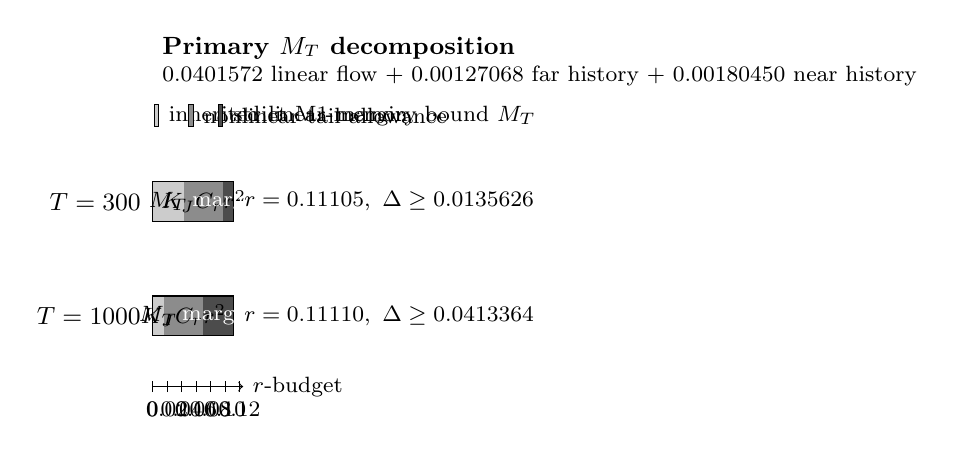
\begin{tikzpicture}[x=9.2cm,y=1cm,every node/.style={font=\footnotesize}]
  % axes
  \draw[->] (0,0.35) -- (0.125,0.35) node[anchor=west] {\(r\)-budget};
  \foreach \x/\lab in {0/0,0.02/0.02,0.04/0.04,0.06/0.06,0.08/0.08,0.10/0.10,0.12/0.12}{
    \draw (\x,0.28)--(\x,0.42);
    \node[below] at (\x,0.28) {\lab};
  }

  \node[anchor=east,font=\small\bfseries] at (-0.003,2.70) {\(T=300\)};
  \node[anchor=east,font=\small\bfseries] at (-0.003,1.25) {\(T=1000\)};

  % T=300 stacked bar
  \fill[black!20] (0,2.45) rectangle (0.0432324134,2.95);
  \fill[black!45] (0.0432324134,2.45) rectangle (0.0974873734,2.95);
  \fill[black!70] (0.0974873734,2.45) rectangle (0.11105,2.95);
  \draw (0,2.45) rectangle (0.11105,2.95);

  % T=1000 stacked bar
  \fill[black!20] (0,1.00) rectangle (0.0154785828,1.50);
  \fill[black!45] (0.0154785828,1.00) rectangle (0.0697636399,1.50);
  \fill[black!70] (0.0697636399,1.00) rectangle (0.11110,1.50);
  \draw (0,1.00) rectangle (0.11110,1.50);

  % labels on bars
  \node[align=center] at (0.0216,2.70) {\(M_T\)};
  \node[align=center] at (0.07036,2.70) {\(K_JC_rr^2\)};
  \node[align=center,text=white] at (0.10427,2.70) {margin};

  \node[align=center] at (0.00774,1.25) {\(M_T\)};
  \node[align=center] at (0.04262,1.25) {\(K_JC_rr^2\)};
  \node[align=center,text=white] at (0.09043,1.25) {margin};

  % numeric annotations
  \node[anchor=west] at (0.1130,2.70)
    {\(r=0.11105,\ \Delta\ge0.0135626\)};
  \node[anchor=west] at (0.1130,1.25)
    {\(r=0.11110,\ \Delta\ge0.0413364\)};

  % legend
  \draw[fill=black!20] (0.002,3.65) rectangle (0.008,3.93);
  \node[anchor=west] at (0.009,3.79) {inherited linear-memory bound \(M_T\)};
  \draw[fill=black!45] (0.050,3.65) rectangle (0.056,3.93);
  \node[anchor=west] at (0.057,3.79) {nonlinear tail allowance};
  \draw[fill=black!70] (0.091,3.65) rectangle (0.097,3.93);
  \node[anchor=west] at (0.098,3.79) {strict M1 margin};

  % term decomposition mini panel
  \node[anchor=west,font=\small\bfseries] at (0,4.65)
    {Primary \(M_T\) decomposition};
  \node[anchor=west] at (0,4.30)
    {\(0.0401572\) linear flow \(+\ 0.00127068\) far history \(+\ 0.00180450\) near history};
\end{tikzpicture}
}
  \caption{Certified memory-tail budgets for the primary and redundant cuts.  Each bar partitions the radius \(r\) into the inherited linear-memory term \(M_T\), the nonlinear tail allowance \(K_JC_rr^2\), and the remaining strict margin.  The top annotation gives the certified decomposition of \(M_T\) for the primary \(T=300\) proof.}
  \label{fig:memory-tail-budget}
\end{figure}

\subsection{Arithmetic model}
\label{subsec:arithmetic-model}

The current certificate combines exact-rational model data and Arb ball arithmetic with selected binary64 layers for the large \(O(N^2)\) matrix and positive-sum computations. The latter carry explicit operation-count and roundoff allowances. The TASK-0006 certificate additionally assumes a few-ulp model for selected elementary \texttt{libm} calls used in the large-kernel layer.

Accordingly, until the publication-hardening rerun is complete, the result is described as a \emph{computer-assisted theorem under the stated IEEE-754/libm arithmetic model}, rather than as an end-to-end interval-arithmetic proof. The arithmetic-hardening computation replaces the remaining load-bearing elementary-function evaluations by verified enclosures without changing the mathematical fixed-point argument.
